
\subsection{Motion R-CNN}
\label{ssec:model}

Building on Mask R-CNN \cite{MaskRCNN},
we estimate per-object motion by predicting the 3D motion of each detected object.
For this, we extend Mask R-CNN in two straightforward ways.
First, we modify the backbone network and provide two frames to the R-CNN system
in order to enable image matching between the consecutive frames.
Second, we extend the Mask R-CNN RoI head to predict a 3D motion for each
region proposal. Tables \ref{table:motionrcnn_resnet} and \ref{table:motionrcnn_resnet_fpn}
show our Motion R-CNN networks based on Mask R-CNN  and Mask R-CNN -FPN,
respectively.

{\begin{table}[h]
\centering
\begin{tabular}{llr}
\toprule
\textbf{Output} & \textbf{Layer Operations} & \textbf{Output Dimensions} \\
\midrule\midrule
& input images & H $\times$ W $\times$ C \\
\midrule
C$_4$ & ResNet \{up to C$_4$\} (Table \ref{table:resnet}) & $\tfrac{1}{16}$ H $\times$ $\tfrac{1}{16}$ W $\times$ 1024 \\
\midrule
\multicolumn{3}{c}{\textbf{Region Proposal Network (RPN)} (Table \ref{table:maskrcnn_resnet})}\\
\midrule
\multicolumn{3}{c}{\textbf{Camera Motion Network}}\\
\midrule
& From C$_4$: ResNet \{C$_6$\} (Table \ref{table:resnet}) & $\tfrac{1}{64}$ H $\times$ $\tfrac{1}{64}$ W $\times$ 2048 \\
& bilinear resize, 7 $\times$ 7 & 7 $\times$ 7 $\times$ 512 \\
& flatten & 1 $\times$ 7 $\cdot$ 7 $\cdot$ 512 \\
T$_0$ & $\begin{bmatrix}\textrm{fully connected}, 1024\end{bmatrix}$ $\times$ 2  & 1 $\times$ 1024 \\

$R_t^{cam}$& From T$_0$: fully connected, 3 & 1 $\times$ 3 \\
$t_t^{cam}$& From T$_0$: fully connected, 3 & 1 $\times$ 3 \\
& From T$_0$: fully connected, 2 & 1 $\times$ 2 \\
$o_t^{cam}$& softmax, 2 & 1 $\times$ 2 \\
\midrule
\multicolumn{3}{c}{\textbf{RoI Head \& RoI Head: Masks} (Table \ref{table:maskrcnn_resnet})}\\
\midrule
\multicolumn{3}{c}{\textbf{RoI Head: Motions}}\\
\midrule
%& From M$_0$: flatten & N$_{RoI}$ $\times$ 7 $\cdot$ 7 $\cdot$ 256 \\
T$_1$ & From ave: $\begin{bmatrix}\textrm{fully connected}, 1024\end{bmatrix}$ $\times$ 2 & N$_{RoI}$ $\times$ 1024 \\
$\forall k: R_t^k$ & From T$_1$: fully connected, 3 & N$_{RoI}$ $\times$ 3 \\
$\forall k: t_t^k$ & From T$_1$: fully connected, 3 & N$_{RoI}$ $\times$ 3 \\
$\forall k: p_t^k$ & From T$_1$: fully connected, 3 & N$_{RoI}$ $\times$ 3 \\
& From T$_1$: fully connected, 2 & N$_{RoI}$ $\times$ 2 \\
$\forall k: o_t^k$ & softmax, 2 & N$_{RoI}$ $\times$ 2 \\

\bottomrule
\end{tabular}

\caption {
Motion R-CNN ResNet architecture based on the Mask R-CNN
ResNet architecture (Table \ref{table:maskrcnn_resnet}).
We use ReLU activations after all hidden layers and
additonally dropout with $p = 0.5$ after all fully-connected hidden layers.
}
\label{table:motionrcnn_resnet}
\end{table}
}

{
\begin{table}[h]
\centering
\begin{tabular}{llr}
\toprule
\textbf{Output} & \textbf{Layer Operations} & \textbf{Output Dimensions} \\
\midrule\midrule
& input images & H $\times$ W $\times$ C \\
\midrule
C$_6$ & ResNet (Table \ref{table:resnet}) & $\tfrac{1}{64}$ H $\times$ $\tfrac{1}{64}$ W $\times$ 2048 \\
\midrule
\multicolumn{3}{c}{\textbf{RPN \& FPN} (Table \ref{table:maskrcnn_resnet_fpn})} \\
\midrule
\multicolumn{3}{c}{\textbf{Camera Motion Network}}\\
\midrule
& From C$_6$: 1 $\times$ 1 conv, 512 & $\tfrac{1}{32}$ H $\times$ $\tfrac{1}{32}$ W $\times$ 512 \\
& bilinear resize, 7 $\times$ 7 & 7 $\times$ 7 $\times$ 512 \\
& flatten & 1 $\times$ 7 $\cdot$ 7 $\cdot$ 512 \\
T$_2$ & $\begin{bmatrix}\textrm{fully connected}, 1024\end{bmatrix}$ $\times$ 2  & 1 $\times$ 1024 \\
$R_t^{cam}$& From T$_2$: fully connected, 3 & 1 $\times$ 3 \\
$t_t^{cam}$& From T$_2$: fully connected, 3 & 1 $\times$ 3 \\
& From T$_2$: fully connected, 2 & 1 $\times$ 2 \\
$o_t^{cam}$& softmax, 2 & 1 $\times$ 2 \\
\midrule
\multicolumn{3}{c}{\textbf{RoI Head \& RoI Head: Masks} (Table \ref{table:maskrcnn_resnet_fpn})} \\
\midrule
\multicolumn{3}{c}{\textbf{RoI Head: Motions}}\\
\midrule
%& From M$_1$: flatten & N$_{RoI}$ $\times$ 14 $\cdot$ 14 $\cdot$ 256 \\
T$_3$ & From F$_1$: $\begin{bmatrix}\textrm{fully connected}, 1024\end{bmatrix}$ $\times$ 2 & N$_{RoI}$ $\times$ 1024 \\
$\forall k: R_t^k$ & From T$_3$: fully connected, 3 & N$_{RoI}$ $\times$ 3 \\
$\forall k: t_t^k$ & From T$_3$: fully connected, 3 & N$_{RoI}$ $\times$ 3 \\
$\forall k: p_t^k$ & From T$_3$: fully connected, 3 & N$_{RoI}$ $\times$ 3 \\
& From T$_2$: fully connected, 2 & N$_{RoI}$ $\times$ 2 \\
$\forall k: o_t^k$ & softmax, 2 & N$_{RoI}$ $\times$ 2 \\

\bottomrule
\end{tabular}

\caption {
Motion R-CNN ResNet-FPN architecture based on the Mask R-CNN
ResNet-FPN architecture (Table \ref{table:maskrcnn_resnet_fpn}).
To obtain a larger bottleneck stride, we compute the feature pyramid starting
with C$_6$ instead of C$_5$ (thus, the subsampling from P$_5$ to P$_6$) is omitted.
The modifications are analogous to our Motion R-CNN ResNet,
but we still show the architecture for completeness.
Again, we use ReLU activations after all hidden layers and
additonally dropout with $p = 0.5$ after all fully-connected hidden layers.
}
\label{table:motionrcnn_resnet_fpn}
\end{table}
}

\paragraph{Motion R-CNN backbone}
Like Faster R-CNN and Mask R-CNN, we use a ResNet \cite{ResNet} variant as backbone network to compute feature maps from input imagery.

Inspired by FlowNetS \cite{FlowNet}, we make one modification to the ResNet backbone to enable image matching,
laying the foundation for our motion estimation. Instead of taking a single image as input to the backbone,
we depth-concatenate two temporally consecutive frames $I_t$ and $I_{t+1}$, yielding a input image map with six channels.
Alternatively, we also experiment with concatenating the camera space XYZ coordinates for each frame,
XYZ$_t$ and XYZ$_{t+1}$, into the input as well.
We do not introduce a separate network for computing region proposals and use our modified backbone network
as both first stage RPN and second stage feature extractor for extracting the RoI features.
Technically, our feature encoder network will have to learn a motion representation similar to
that learned by the FlowNet encoder, but the output will be computed in the
object-centric framework of a region based convolutional network head with a 3D parametrization.
Thus, in contrast to the dense FlowNet decoder, the estimated dense motion information
from the encoder is integrated for specific objects via RoI cropping and
processed by the RoI head for each object.

\paragraph{Per-RoI motion prediction}
We use a rigid 3D motion parametrization similar to the one used in SfM-Net and SE3-Nets \cite{SfmNet,SE3Nets}.
For the $k$-th object proposal, we predict the rigid transformation $\{R_t^k, t_t^k\}\in \mathbf{SE}(3)$
\footnote{$\mathbf{SE}(3)$ refers to the Special Euclidean Group representing 3D rotations
and translations: $\{R, t|R \in \mathbf{SO}(3), t \in \mathbb{R}^3\}$}
of the object between the two frames $I_t$ and $I_{t+1}$, as well as the object pivot $p_t^k \in \mathbb{R}^3$ at time $t$.
We parametrize ${R_t^k}$ using an Euler angle representation,

\begin{equation}
R_t^k = R_t^{k,z}(\gamma) \cdot R_t^{k,x}(\alpha) \cdot R_t^{k,y}(\beta),
\end{equation}

where
\begin{equation}
R_t^{k,x}(\alpha) =
\begin{pmatrix}
  1 & 0 & 0 \\
  0 & \cos(\alpha) & -\sin(\alpha) \\
  0 & \sin(\alpha) & \cos(\alpha)
\end{pmatrix},
\end{equation}

\begin{equation}
R_t^{k,y}(\beta) =
\begin{pmatrix}
  \cos(\beta) & 0 & \sin(\beta) \\
  0 & 1 & 0 \\
  -\sin(\beta) & 0 & \cos(\beta)
\end{pmatrix},
\end{equation}

\begin{equation}
R_t^{k,z}(\gamma) =
\begin{pmatrix}
  \cos(\gamma) & -\sin(\gamma) & 0 \\
  \sin(\gamma) & \cos(\gamma) & 0 \\
  0 & 0 & 1
\end{pmatrix},
\end{equation}

and $\alpha, \beta, \gamma$ are the rotation angles in radians about the $x,y,z$-axis, respectively.

We then extend the Mask R-CNN head by adding a small fully-connected network for motion
prediction in addition to the fully-connected layers for
refined boxes and classes and the convolutional network for the masks.
Like for refined boxes and masks, we make one separate motion prediction for each class.
Each instance motion is predicted as a set of nine scalar parameters,
$\sin(\alpha)$, $\sin(\beta)$, $\sin(\gamma)$, $t_t^k$ and $p_t^k$,
where $\sin(\alpha)$, $\sin(\beta)$ and $\sin(\gamma)$ are clipped to $[-1, 1]$.
Here, we assume that motions between frames are relatively small
and that objects rotate at most 90 degrees in either direction along any axis,
which is in general a safe assumption for image sequences from videos.
All predictions are made in camera space, and translation and pivot predictions are in meters.
We additionally predict softmax scores $o_t^k$ for classifying the objects into
still and moving objects. As a postprocessing, for any object instance $k$ with predicted moving flag $o_t^k = 0$,
we set $\sin(\alpha) = \sin(\beta) = \sin(\gamma) = 0$ and $t_t^k = (0,0,0)^T$,
and thus predict an identity motion.


\paragraph{Camera motion prediction}
In addition to the object transformations, we optionally predict the camera motion $\{R_t^{cam}, t_t^{cam}\}\in \mathbf{SE}(3)$
between the two frames $I_t$ and $I_{t+1}$.
For this, we branch off a small fully-connected network from the bottleneck output of the backbone.
We again represent $R_t^{cam}$ using a Euler angle representation and
predict $\sin(\alpha)$, $\sin(\beta)$, $\sin(\gamma)$ and $t_t^{cam}$ in the same way as for the individual objects.
Again, we predict a softmax score $o_t^{cam}$ for differentiating between
a still and moving camera.

\subsection{Network design}

\label{ssec:design}
\paragraph{Camera motion network}
In our  variant (Table \ref{table:motionrcnn_resnet}), the underlying
ResNet backbone is only computed up to the $C_4$ block, as otherwise the
feature resolution prior to RoI extraction would be reduced too much.
In our  variant, we therefore first pass the $C_4$ features through a $C_5$
block to make the camera network of both variants comparable.
Then, in both, the  and -FPN variant (Table \ref{table:motionrcnn_resnet_fpn}), we apply a additional
convolution to the $C_5$ features to reduce the number of inputs to the following
fully-connected layers.
Instead of averaging, we use bilinear resizing to bring the convolutional features
to a fixed size without losing all spatial information,
flatten them, and finally apply multiple fully-connected layers to compute the
camera motion prediction.

\paragraph{RoI motion head network}
In both of our network variants
(Tables \ref{table:motionrcnn_resnet} and \ref{table:motionrcnn_resnet_fpn}),
we compute the fully-connected network for motion prediction from the
flattened RoI features, which are also the basis for classification and
bounding box refinement.

\subsection{Supervision}
\label{ssec:supervision}

\paragraph{Per-RoI instance motion supervision with 3D instance motion ground truth}
The most straightforward way to supervise the object motions is by using ground truth
motions computed from ground truth object poses, which is in general
only practical when training on synthetic datasets.
Given the $k$-th foreground RoI, let $i_k$ be the index of the matched ground truth example with class $c_k^*$,
let $R^{k,c_k}, t^{k,c_k}, p^{k,c_k}, o^{k,c_k}$ be the predicted motion for class $c_k^*$
and $R^{gt,i_k}, t^{gt,i_k}, p^{gt,i_k}, o^{gt,i_k}$ the ground truth motion for the example $i_k$.
Note that we dropped the subscript $t$ to increase readability.
Similar to the camera pose regression loss in \cite{PoseNet2},
we use a variant of the $\ell_1$-loss to penalize the differences between ground truth and predicted
rotation, translation (and pivot, in our case). We found that the smooth $\ell_1$-loss
performs better in our case than the standard $\ell_1$-loss.
We then compute the RoI motion loss as

\begin{equation}
L_{motion} = \frac{1}{N_{RoI}^{fg}} \sum_k^{N_{RoI}} l_{p}^k + (l_{R}^k + l_{t}^k) \cdot o^{gt,i_k} + l_o^k,
\end{equation}
where
\begin{equation}
l_{R}^k = \ell_{reg} (R^{gt,i_k} - R^{k,c_k}),
\end{equation}
\begin{equation}
l_{t}^k = \ell_{reg} (t^{gt,i_k} - t^{k,c_k}),
\end{equation}
\begin{equation}
l_{p}^k = \ell_{reg} (p^{gt,i_k} - p^{k,c_k}).
\end{equation}
are the smooth $\ell_1$-loss terms for the predicted rotation, translation and pivot,
respectively and
\begin{equation}
l_o^k = \ell_{cls}(o_t^k, o^{gt,i_k}).
\end{equation}
is the cross-entropy loss for the predicted classification into moving and non-moving objects.

Note that we do not penalize the rotation and translation for objects with
$o^{gt,i_k} = 0$, which do not move between $t$ and $t+1$. We found that the network
may not reliably predict exact identity motions for still objects, which is
numerically more difficult to optimize than performing classification between
moving and non-moving objects and discarding the regression for the non-moving
ones. Also, analogous to masks and bounding boxes, the estimates for classes
other than $c_k^*$ are not penalized.

Now, our modified RoI loss is
\begin{equation}
L_{RoI} = L_{cls} + L_{box} + L_{mask} + L_{motion}.
\end{equation}

\paragraph{Camera motion supervision}
We supervise the camera motion with ground truth analogously to the
object motions, with the only difference being that we only have
a rotation and translation, but no pivot term for the camera motion.
If the ground truth shows that the camera is not moving, we again do not
penalize rotation and translation. For the camera, the loss is reduced to the
classification term in this case.

\paragraph{Per-RoI instance motion supervision \emph{without} 3D instance motion ground truth}
\begin{figure}[t]
  \centering
  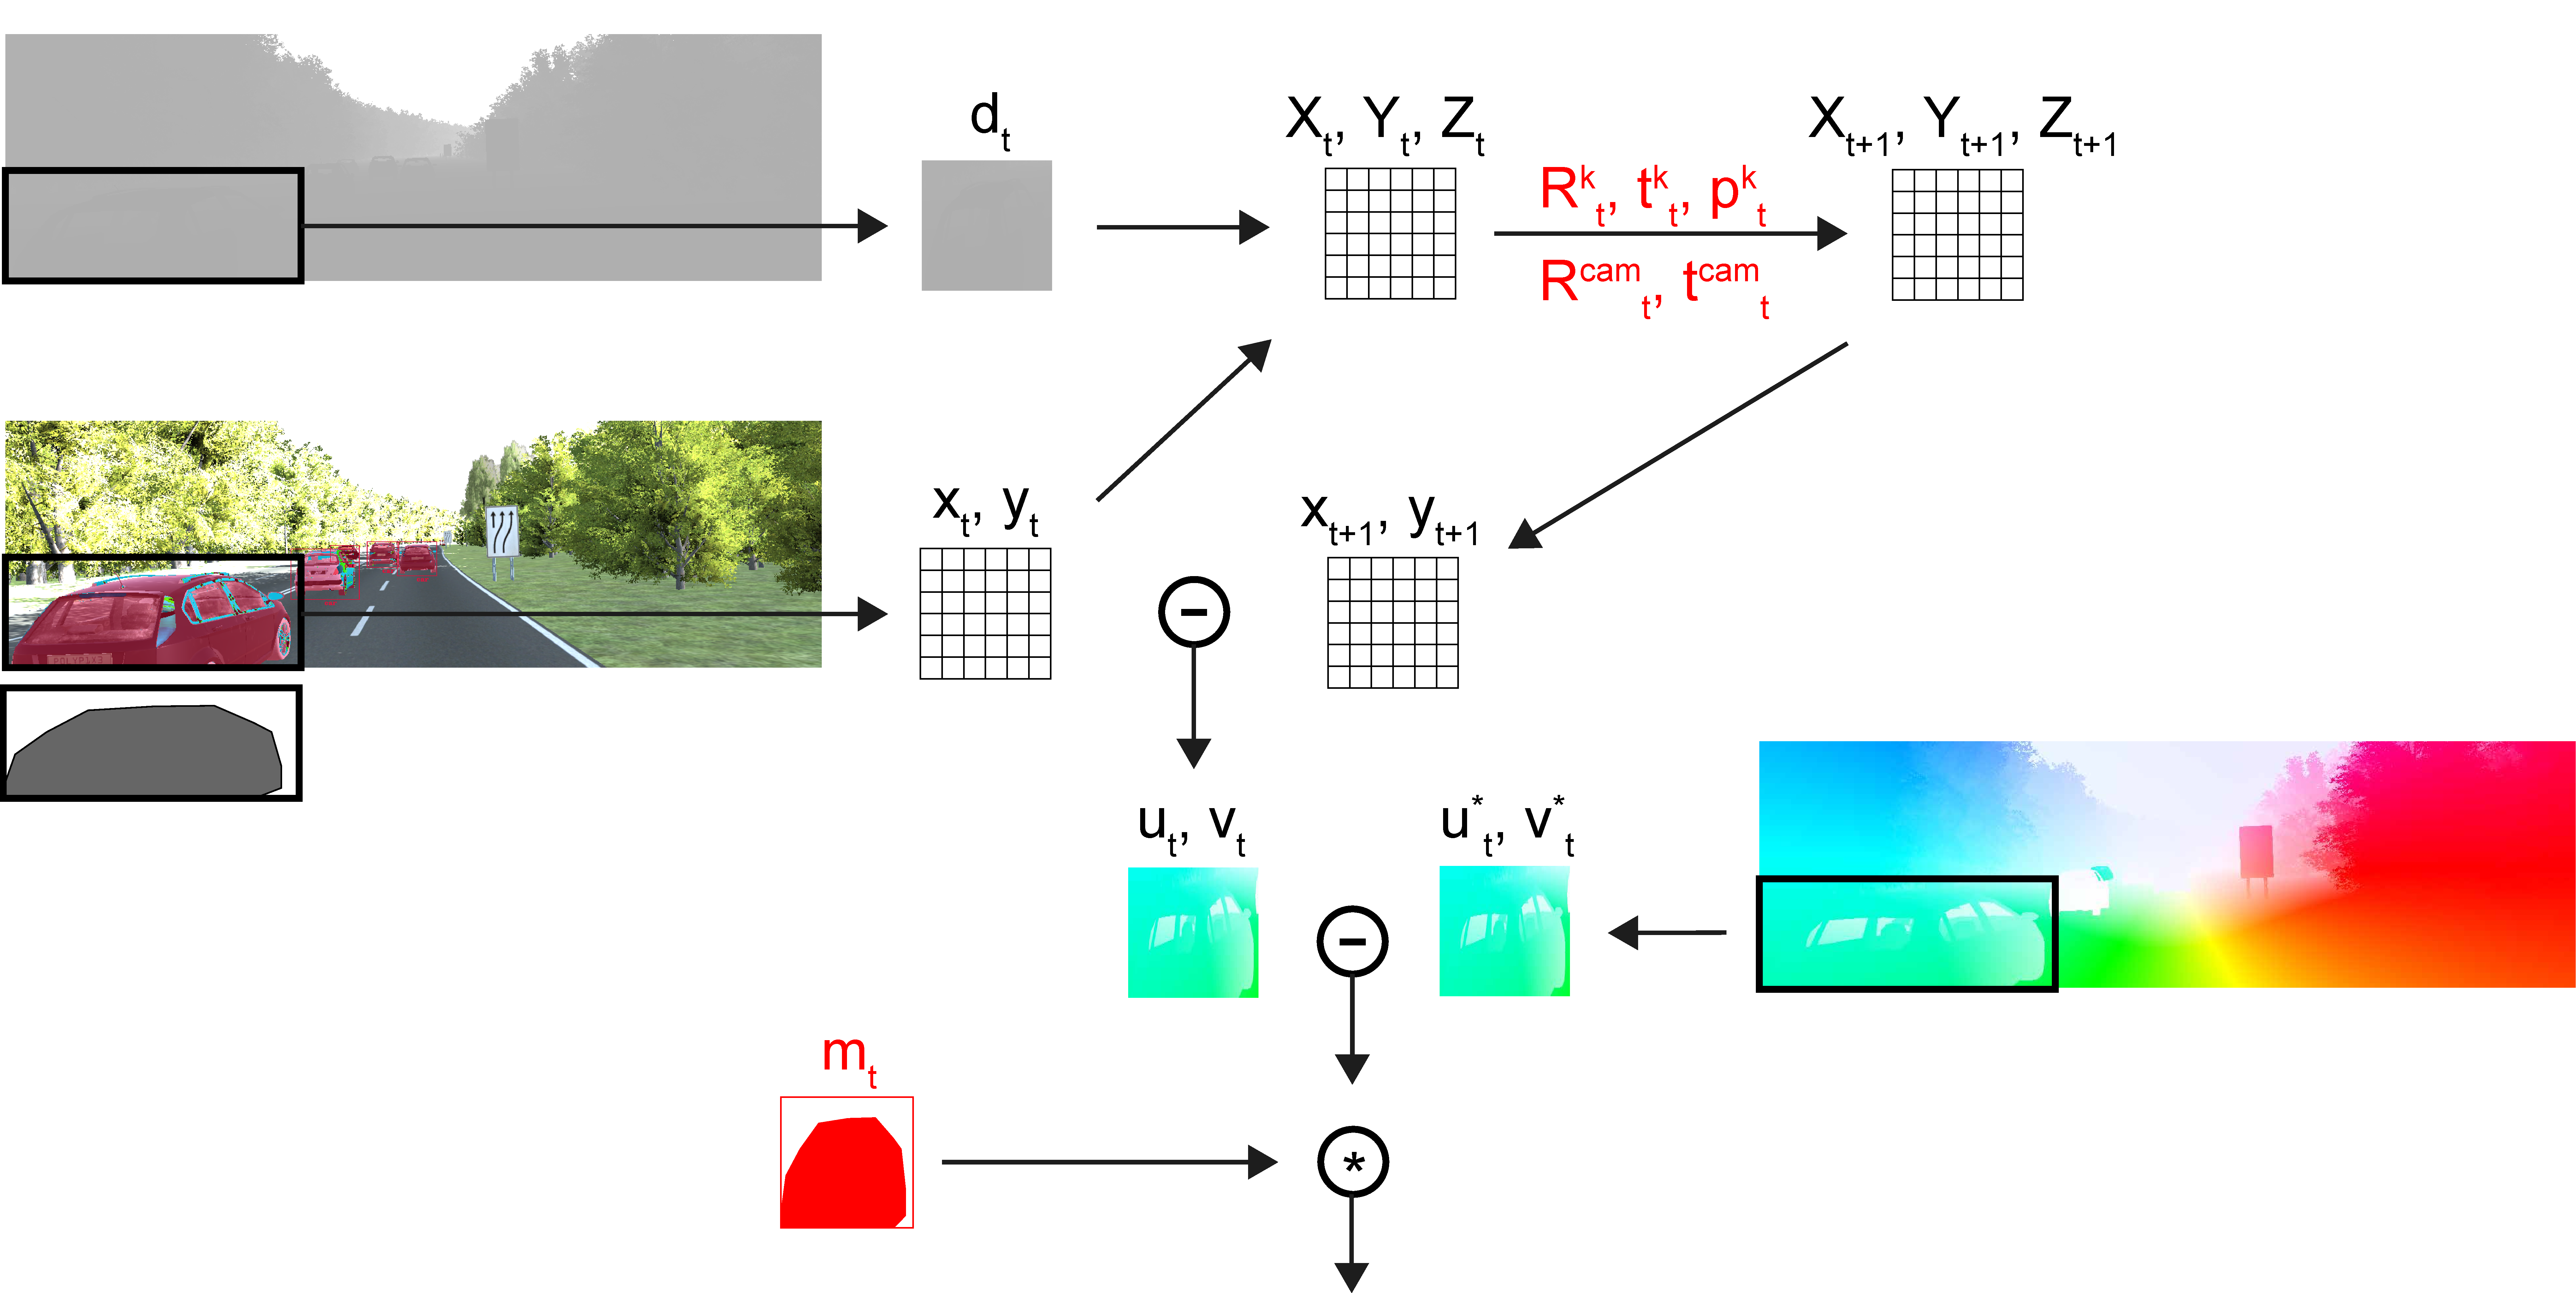
\includegraphics[width=\textwidth]{figures/flow_loss}
\caption{
Overview of the alternative, optical flow based loss for instance motion
supervision without 3D instance motion ground truth.
In contrast to SfM-Net, where a single optical flow field is
composed and penalized to supervise the motion prediction, our loss considers
the motion of all objects in isolation and composes a batch of flow windows
for the RoIs.
}
\label{figure:flow_loss}
\end{figure}

A more general way to supervise the object motions is a re-projection
loss similar to the unsupervised loss in SfM-Net \cite{SfmNet},
which we can apply to coordinates within the object bounding boxes,
and which does not require ground truth 3D object motions.

In this case, for any RoI,
we generate a uniform $m \times m$ 2D grid of points inside the RPN proposal bounding box
with the same resolution as the predicted mask.
We use the same bounding box
to crop the corresponding region from the dense, full image depth map
and bilinearly resize the depth crop to the same resolution as the mask and point
grid.
We then compute the optical flow at each of the grid points by creating
a 3D point cloud from the point grid and depth crop. To this point cloud, we
apply the RoI's predicted motion, masked by the predicted mask.
Then, we apply the camera motion to the points, project them back to 2D
and finally compute the optical flow at each point as the difference of the initial and re-projected 2D grids.
Note that we batch this computation over all RoIs, so that we only perform
it once per forward pass. Figure \ref{figure:flow_loss} illustrates the approach.
The mathematical details for the 3D transformations and mappings between 2D and 3D are analogous to the
dense, full image flow composition in the following subsection, so we will not
include them here. The only differences are that there is no sum over objects during
the point transformation based on instance motion, as we consider the single object
corresponding to an RoI in isolation, and that the masks are not resized to the
full image resolution, as
the depth crops and 2D point grid are at the same resolution as the predicted
$m \times m$ mask.

For each RoI, we can now compute $L_{RoI}$ and thus supervise the object motion
by penalizing the $m \times m$ optical flow grid.
If there is optical flow ground truth available, we can use the RoI bounding box to
crop and resize a region from the ground truth optical flow to match the RoI's
optical flow grid and penalize the difference between the flow grids with an $\ell_1$-loss.

However, we can also use the re-projection loss without optical flow ground truth
to train the motion prediction in an unsupervised manner, similar to \cite{SfmNet}.
In this case, we use the bounding box to crop and resize a corresponding region
from the first image $I_t$ and bilinearly sample a region from the second image $I_{t+1}$
using the 2D grid displaced with the predicted flow grid. Then, we can penalize the difference
between the resulting image crops, for example, with a census loss \cite{CensusTerm,UnFlow}.
For more details on differentiable bilinear sampling for deep learning, we refer the reader to
\cite{STN}.

When compared to supervision with motion ground truth, a re-projection
loss could benefit motion regression by removing any loss balancing issues between the
rotation, translation and pivot terms \cite{PoseNet2},
which can make it interesting even when 3D motion ground truth is available.

\subsection{Training and inference}
\label{ssec:training_inference}
\paragraph{Training}
We train the Motion R-CNN RPN and RoI heads in the exact same way as described for Mask R-CNN.
We additionally compute the camera and instance motion losses and concatenate additional
information into the network input, but otherwise do not modify the training procedure
and sample proposals and RoIs in the exact same way.

\paragraph{Inference}
During inference, we proceed analogously to Mask R-CNN.
In the same way as the RoI mask head, at test time, we compute the RoI motion head
from the features extracted with refined bounding boxes.
Additionally, we use the \emph{predicted} binarized masks for each RoI to mask the
extracted RoI features before passing them into the motion head.
The intuition behind that is that we want to mask out (set to zero) any positions in the
extracted feature window which belong to the background. Then, the RoI motion
head aggregates the motion (image matching) information from the backbone
over positions localized within the object only, but not over positions belonging
to the background, which should not influence the final object motion estimate.

Again, as for masks and bounding boxes in Mask R-CNN,
the predicted output object motions are the predicted object motions for the
highest scoring class.

\subsection{Dense flow from motion}
\label{ssec:postprocessing}
As a postprocessing, we compose a dense optical flow map from the outputs of our Motion R-CNN network.
Given the depth map $d_t$ for frame $I_t$, we first create a 3D point cloud in camera space at time $t$,
where
\begin{equation}
P_t =
\begin{pmatrix}
X_t \\ Y_t \\ Z_t
\end{pmatrix}
=
\frac{d_t}{f}
\begin{pmatrix}
x_t - c_0 \\ y_t - c_1 \\ f
\end{pmatrix},
\end{equation}
is the 3D coordinate at $t$ corresponding to the point with pixel coordinates $x_t, y_t$,
which range over all coordinates in $I_t$.
For now, the depth map is always assumed to come from ground truth.

Given $k$ detections with predicted motions as above, we transform all points within the bounding
box of a detected object according to the predicted motion of the object.

We first define the \emph{full image} mask $M_t^k$ for object k,
which can be computed from the predicted box mask $m_t^k$ by bilinearly resizing
$m_t^k$ to the width and height of the predicted bounding box and then copying the values
of the resized mask into a full resolution mask initialized with zeros,
starting at the top-left coordinate of the predicted bounding box.
Then, given the predicted motions $(R_t^k, t_t^k)$ as well as $p_t^k$ for all objects,
\begin{equation}
P'_{t+1} =
P_t + \sum_1^{k} M_t^k\left\{ R_t^k \cdot (P_t - p_t^k) + p_t^k + t_t^k - P_t \right\}
\end{equation}
These motion predictions are understood to have already taken into account
the classification into moving and still objects,
and we thus, as described above, have identity motions for all objects with $o_t^k = 0$.

Next, we transform all points given the camera transformation $\{R_t^c, t_t^c\} \in \mathbf{SE}(3)$,

\begin{equation}
\begin{pmatrix}
X_{t+1} \\ Y_{t+1} \\ Z_{t+1}
\end{pmatrix}
= P_{t+1} = R_t^c \cdot P'_{t+1} + t_t^c
\end{equation}.

Note that in our experiments, we either use the ground truth camera motion to focus
on evaluating the object motion predictions or the predicted camera motion to evaluate
the complete motion estimates. We will always state which variant we use in the experimental section.

Finally, we project the transformed 3D points at time $t+1$ to pixel coordinates again,
\begin{equation}
\begin{pmatrix}
x_{t+1} \\ y_{t+1}
\end{pmatrix}
=
\frac{f}{Z_{t+1}}
\begin{pmatrix}
X_{t+1} \\ Y_{t+1}
\end{pmatrix}
+
\begin{pmatrix}
c_0 \\ c_1
\end{pmatrix}.
\end{equation}
We can now obtain the optical flow between $I_t$ and $I_{t+1}$ at each point as
\begin{equation}
\begin{pmatrix}
u \\ v
\end{pmatrix}
=
\begin{pmatrix}
x_{t+1} - x_{t} \\ y_{t+1} - y_{t}
\end{pmatrix}.
\end{equation}
